\renewcommand*{\arraystretch}{1.1}

\noindent\begin{tabularx}{\queryCardWidth}{|>{\queryPropertyCell}c|X|}
	\hline
	query & Interactive / short / 7 \\ \hline
%
	title & Message Replies \\ \hline
%
    pattern & \hfill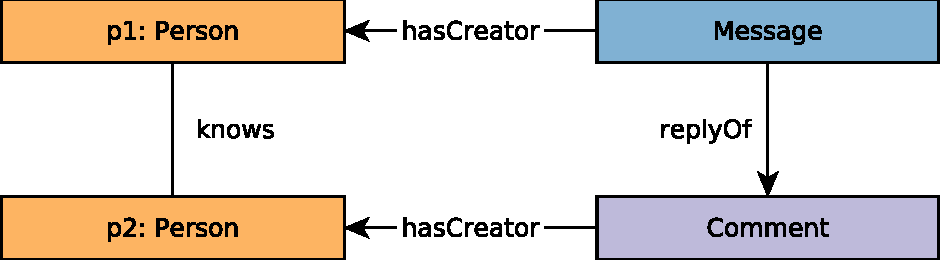
\includegraphics[scale=\patternscale,margin=0cm .2cm]{patterns/interactive-short-read-07}\hfill\vadjust{} \\ \hline
%
	desc. & Given a Message, retrieve the (1-hop) Comments that reply to it.

In addition, return a boolean flag \texttt{knows} indicating if the
author of the reply knows the author of the original message. If author
is same as original author, return false for \texttt{knows} flag.
 \\ \hline
%
	
%
	params &
	\innerCardVSpace{\begin{tabularx}{\attributeCardWidth}{|>{\paramNumberCell}c|>{\varNameCell}M|>{\typeCell}m{\typeWidth}|Y|} \hline
	\cellcolor{parameter} \color{white} \footnotesize $\mathsf{1}$ &Message.id& ID &  \\ \hline
	\end{tabularx}}\innerCardVSpace \\ \hline
%
	
        result &
        \innerCardVSpace{\begin{tabularx}{\attributeCardWidth}{|>{\resultNumberCell}c|>{\varNameCell}M|>{\typeCell}m{\typeWidth}|>{\resultOriginCell}c|Y|} \hline
        $\mathsf{1}$ & Message<-replyOf-Comment.id & ID &R&
                 \\ \hline
        $\mathsf{2}$ & Message<-replyOf-Comment.content & String &R&
                 \\ \hline
        $\mathsf{3}$ & Message<-replyOf-Comment.creationDate & DateTime &R&
                 \\ \hline
        $\mathsf{4}$ & Comment-hasCreator->Person.id & ID &R&
                 \\ \hline
        $\mathsf{5}$ & Comment-hasCreator->Person.firstName & String &R&
                 \\ \hline
        $\mathsf{6}$ & Comment-hasCreator->Person.lastName & String &R&
                 \\ \hline
        $\mathsf{7}$ & knows & Boolean &C&
                original message author knows reply author \\ \hline
        \end{tabularx}}\innerCardVSpace \\ \hline
	
%
	sort        &
        \innerCardVSpace{\begin{tabular}{|>{\sortNumberCell}c|>{\varNameCell}l|>{\directionCell}c|} \hline
        $\mathsf{1}$ & Message<-replyOf-Comment.creationDate & $\desc$ \\ \hline
        $\mathsf{2}$ & Message-hasCreator->Person.id & $\asc$ \\ \hline
        \end{tabular}}\innerCardVSpace \\ \hline
	%
	%
	%
    %
\end{tabularx}
\queryCardVSpace